\documentclass[conference]{IEEEtran}

\usepackage{amsmath}
\usepackage{graphicx}
\usepackage{pgfplots}
\usepackage{tikz}
\usepackage{multirow}
\usepackage{booktabs}
\usepackage{xcolor}
\usepackage{algorithm}
\usepackage{algpseudocode}
\usepackage{listings}
\usepackage{balance}

% Ensure algorithm captions follow IEEE style: "Algorithm 1: Title" (no extra space).
\makeatletter
\renewcommand{\fnum@algorithm}{Algorithm \thealgorithm:}
\makeatother

\pgfplotsset{compat=1.18,
  every axis/.append style={
    label style={font=\footnotesize},
    tick label style={font=\footnotesize},
  }
}
\usetikzlibrary{arrows.meta,positioning,shapes.geometric,fit,calc}

% Improve float separation so adjacent top-of-column tables/figures do not visually merge.
% IEEEtran is already fairly tight; keep enough vertical whitespace so stacked floats don't look fused.
\setlength{\floatsep}{12pt plus 2pt minus 2pt}
\setlength{\textfloatsep}{14pt plus 2pt minus 4pt}
\setlength{\intextsep}{12pt plus 2pt minus 2pt}

\lstset{basicstyle=\ttfamily\footnotesize,breaklines=true,columns=fullflexible}

\title{DT-MR-FALCON: Digital Twin--Assisted Mixed Reality Emergency Corridor Optimization for Intelligent Ambulance Navigation}


\begin{document}

\maketitle

\begin{abstract}
Traffic jams in cities can make it much harder for emergency medical responders to get to the scene of an accident, especially in big cities with a lot of people. Ambulances often have to wait at busy roadways and signalized intersections, which can be very dangerous for patients in emergencies that require immediate attention. Traditional traffic signal control systems use fixed timing strategies and can't change their timing based on the movement of emergency vehicles or the current state of traffic.This paper presents DT-MR-FALCON, a Digital Twin-assisted Mixed Reality framework designed for intelligent ambulance traffic clearance in urban settings. The suggested system combines Digital Twin traffic simulation, Federated Multi-Agent Reinforcement Learning-based traffic signal coordination, edge AI traffic perception, and Mixed Reality navigation to make and show emergency corridors for ambulance drivers in real time. The Digital Twin part models and predicts traffic jams in real time, and the federated reinforcement learning framework coordinates several intersections to cut down on ambulance delays. The Mixed Reality navigation interface helps drivers get through complicated traffic situations by showing them the layout of the corridor and keeping them aware of what's going on around them in real time.
We use the Simulation of Urban Mobility traffic simulator to test the proposed framework on a number of real-world urban traffic datasets, using multiple metropolis-scale urban road networks extracted from OpenStreetMap. Experimental results show that the suggested method cuts down on ambulance travel time, intersection delay, and traffic congestion by a large amount compared to standard signal control methods. Simulation results show that DT-MR-FALCON reduces ambulance travel time by approximately 46\% and decreases average intersection delay by about 35\% compared with fixed-time traffic signal control. These findings underscore the potential of amalgamating Digital Twin technology, artificial intelligence, and Mixed Reality navigation for advanced intelligent transportation systems.
\end{abstract}

\begin{IEEEkeywords}
Emergency Vehicle Navigation, Intelligent Transportation Systems, Digital Twin Traffic Modeling, Mixed Reality Navigation, Federated Multi-Agent Reinforcement Learning, Traffic Signal Optimization, Edge AI Traffic Perception, Vehicle-to-Infrastructure Communication
\end{IEEEkeywords}

\section{Introduction}
Traffic jams in cities have become a big problem for emergency medical response systems in modern cities. Rapid urbanization and a steady rise in the number of cars owned have made traffic in cities around the world much denser. Ambulances often have to wait longer than usual to get through intersections and busy traffic corridors in multiple metropolis-scale urban road networks extracted from OpenStreetMap. These delays have a direct effect on emergency medical services and could lower the chances of patients surviving in situations where time is of the essence.Most traditional traffic signal control systems use fixed-time scheduling or rule-based control systems to work. These methods do control the flow of traffic in general, but they can't change based on real-time traffic conditions or the movement of emergency vehicles. Because of this, ambulances often have to wait a long time at signalized intersections and run into traffic jams that are hard to predict.Recent advancements in Intelligent Transportation Systems (ITS) have investigated the application of artificial intelligence and machine learning methodologies to enhance urban traffic management. Reinforcement learning-based traffic signal control has shown great promise in improving traffic flow on city networks. Multi-agent traffic control systems let intersections work together and change their signal phases based on what they see happening on the road in real time. Digital Twin technology has also become a powerful way to model and simulate urban environments by making virtual copies of real-world.Even with these improvements, most current traffic optimization frameworks still focus mainly on controlling traffic at the infrastructure level and don't help emergency vehicle drivers very much. Most ambulance navigation systems today use regular GPS routing, which doesn't take into account changing traffic patterns and doesn't visually guide drivers through the best traffic routes.To overcome these constraints, this paper introduces DT-MR-FALCON, a Digital Twin-assisted Mixed Reality framework aimed at enhancing emergency vehicle mobility in densely populated urban settings. The suggested system combines Digital Twin traffic prediction, Federated Multi-Agent Reinforcement Learning for coordinated traffic signal control, edge AI traffic perception, and Mixed Reality visualization to dynamically create emergency corridors for ambulance drivers.
The main contributions of this work are summarized as follows:

\noindent 1) A framework for modeling traffic using Digital Twins that can predict how traffic will change in real time on large urban road networks.

\noindent 2) A federated multi-agent reinforcement learning signal coordination method that improves signal control at many intersections and cuts down on the time it takes for emergency vehicles to get to their destinations.

\noindent 3) A Mixed Reality navigation interface that overlays a dynamic emergency corridor within the driver’s field of view to improve situational awareness and navigation efficiency.

\noindent 4) A large-scale, multi-city simulation test of the proposed DT-MR-FALCON framework on different types of urban road networks, showing that it can work in a variety of traffic situations.
\noindent As far as we know, this is the first framework that combines Digital Twin traffic prediction, federated multi-agent reinforcement learning traffic signal control, and Mixed Reality navigation help for making dynamic emergency corridors in city traffic networks.

\section{Related Work}
Recent studies in intelligent transportation systems have examined various strategies to enhance traffic signal management and facilitate emergency vehicle movement in urban settings. Conventional traffic signal control methods depend on fixed-time or actuated signal scheduling, which cannot adjust to changing traffic conditions in real time. As urban transportation networks get more complicated, these static control systems are no longer enough to handle traffic jams and give emergency vehicles priority.Machine learning techniques, particularly reinforcement learning, have recently gained attention for adaptive traffic signal optimization \cite{b1,b2,b3,b5}. Traffic control systems that use reinforcement learning let intersections learn the best signal policies by interacting with traffic environments. Multi-agent reinforcement learning approaches take this idea even further by letting multiple intersections work together and coordinate signal phases to make traffic flow more smoothly across city networks. \cite{b9}.The proposed DT-MR-FALCON system, on the other hand, combines Digital Twin traffic prediction and Mixed Reality driver assistance to directly help emergency vehicles find their way and optimize corridors. This is different from current reinforcement-learning traffic signal control systems that mostly focus on improving traffic flow at intersections.
Another emerging concept in smart city infrastructure is the use of Digital Twin technology \cite{b13,b14,b15,b16}. A Digital Twin is a virtual model of a real system that gets real-time data from sensors and connected devices all the time. Digital Twin models can simulate traffic conditions and predict patterns of congestion across road networks in the context of transportation systems. This ability to predict traffic allows for proactive traffic management plans that plan for congestion before it happens.In parallel, advancements in connected vehicle technology have enabled Vehicle-to-Infrastructure communication between vehicles and traffic management systems \cite{b25,b26}. These kinds of communication systems let traffic signals see emergency vehicles coming and change the phases of the signals as needed. But a lot of the current methods focus mostly on optimizing traffic on the infrastructure side and don't do much to help emergency vehicle drivers.Recent advancements in augmented reality and mixed reality navigation systems have shown promise in enhancing driver awareness by superimposing digital information onto the physical environment \cite{b27,b28}. Mixed Reality technologies can show navigation paths, obstacles, and spatial guidance cues in real time, which can help drivers be more aware of their surroundings in complicated situations.Even with these improvements, most research still looks at these technologies separately. Traffic control systems that use reinforcement learning focus on optimizing signals, digital twin models focus on predictive simulation, and mixed reality navigation systems focus on helping drivers in general. There aren't many frameworks that combine predictive traffic modeling, distributed traffic signal coordination, and real-time Mixed Reality navigation into one system that is specifically made for emergency vehicle operations.To fill this gap, the proposed DT-MR-FALCON framework uses Digital Twin traffic prediction, Federated Multi-Agent Reinforcement Learning traffic signal coordination, and Mixed Reality navigation assistance to make emergency corridors on the fly and make it easier for ambulances to get around in busy city traffic networks.

\section{System Architecture}
The proposed DT-MR-FALCON framework combines different smart transportation technologies to make it possible for ambulances to find their way by creating dynamic emergency corridors. The system uses Digital Twin traffic modeling, Federated Multi-Agent Reinforcement Learning traffic signal control, edge AI perception, and Mixed Reality navigation to make an intelligent transportation architecture that can adapt to changing traffic conditions in real time. Fig.~\ref{fig:architecture} summarizes the end-to-end data and control flow across sensing, prediction, optimization, actuation, and in-vehicle visualization.

\begin{figure}[t]
\centering
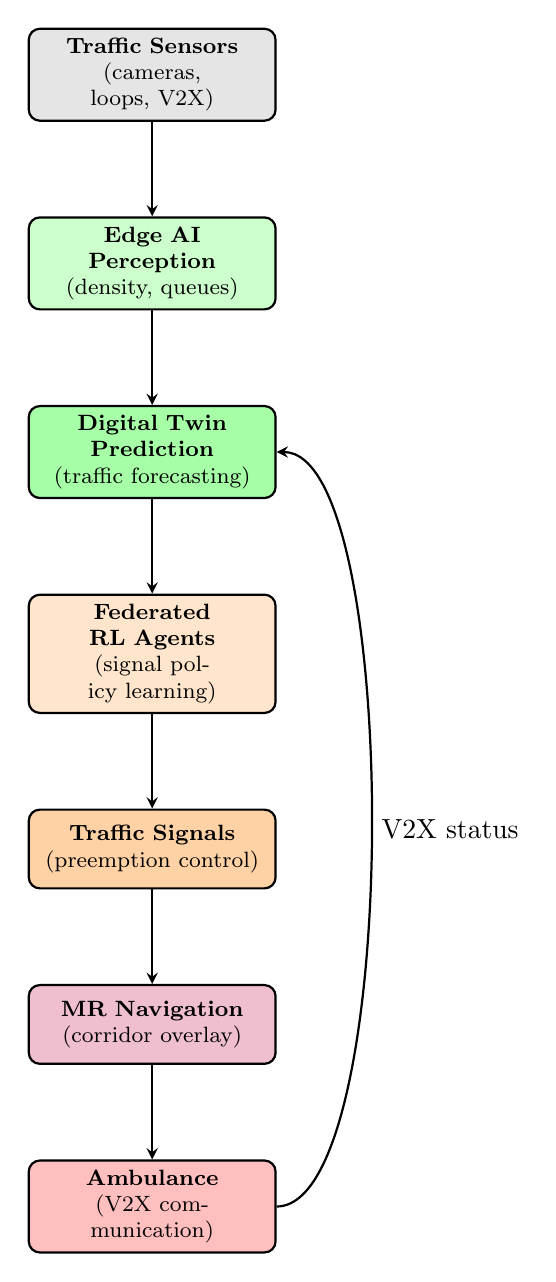
\begin{tikzpicture}[node distance=1.2cm,>=stealth]

\tikzstyle{block}=[
  rectangle,
  draw,
  thick,
  rounded corners,
  text width=2.9cm,
  minimum height=1.0cm,
  align=center,
  font=\footnotesize
]

\node[block, fill=gray!20] (sensor)
{\textbf{Traffic Sensors}\\(cameras, loops, V2X)};

\node[block, fill=green!20, below=1.2cm of sensor] (edge)
{\textbf{Edge AI Perception}\\(density, queues)};

\node[block, fill=green!35, below=1.2cm of edge] (dt)
{\textbf{Digital Twin Prediction}\\(traffic forecasting)};

\node[block, fill=orange!20, below=1.2cm of dt] (rl)
{\textbf{Federated RL Agents}\\(signal policy learning)};

\node[block, fill=orange!35, below=1.2cm of rl] (sig)
{\textbf{Traffic Signals}\\(preemption control)};

\node[block, fill=purple!25, below=1.2cm of sig] (mr)
{\textbf{MR Navigation}\\(corridor overlay)};

\node[block, fill=red!25, below=1.2cm of mr] (amb)
{\textbf{Ambulance}\\(V2X communication)};

% Vertical arrows
\draw[->, thick] (sensor) -- (edge);
\draw[->, thick] (edge) -- (dt);
\draw[->, thick] (dt) -- (rl);
\draw[->, thick] (rl) -- (sig);
\draw[->, thick] (sig) -- (mr);
\draw[->, thick] (mr) -- (amb);

% Feedback arrow
\draw[->, thick]
(amb.east) .. controls +(1.6cm,0) and +(1.6cm,0) ..
node[right]{V2X status}
(dt.east);

\end{tikzpicture}

\caption{Overview of the DT-MR-FALCON system architecture integrating sensing, Digital Twin prediction, federated RL coordination, and Mixed Reality ambulance guidance.}
\label{fig:architecture}
\end{figure}

The system architecture as a whole is made up of several parts that work together to sense, predict, optimize, and visualize. Traffic data is gathered via distributed sensing infrastructure, including roadside cameras, connected vehicles, and traffic sensors. Edge computing modules process these data streams to figure out how many cars are on the road, how fast they are going, and how long the lines are at intersections. The Digital Twin traffic simulation layer, which keeps a virtual model of the city's traffic network, then gets the processed traffic state data.The Digital Twin model keeps track of its state in real time by using traffic observations and makes short-term predictions about how traffic will change across the road network. The Federated Multi-Agent Reinforcement Learning module uses these predictions to figure out the best ways to control traffic signals so that ambulances don't have to wait too long while still keeping traffic moving smoothly for other cars. Each intersection functions as an independent entity that acquires traffic signal strategies while coordinating with adjacent intersections via federated parameter updates.
At the same time, the system finds the best emergency corridor for the ambulance that is on its way by looking at predicted traffic patterns and current traffic conditions. Once the best route is found, traffic lights along the chosen corridor are automatically adjusted to give ambulances the most priority.The Mixed Reality navigation interface shows the ambulance driver the computed emergency corridor right on top of what they can see, giving them real-time directions. This visualization helps the driver see the best way to get through heavy traffic while still being aware of other cars and obstacles around them.The architecture makes it easy for sensing infrastructure, predictive traffic modeling, distributed traffic signal control, and driver assistance systems to work together.

\subsection{Emergency Corridor Generation Framework}
DT-MR-FALCON generates an emergency corridor through a closed-loop pipeline: (i) the Digital Twin predicts short-horizon congestion, (ii) the corridor optimizer selects a congestion-aware path, (iii) federated multi-agent signal coordination aligns green phases along the selected corridor, and (iv) the Mixed Reality interface visualizes the corridor and guidance cues for the driver.
Given a candidate corridor (path) $P$ composed of road segments $e \in P$, the corridor optimization objective is formulated as

\begin{equation}
C^{*} = \arg\min_{P} \sum_{e \in P} (T_e + \lambda D_e)
\end{equation}

where $T_e$ denotes the predicted traversal time of segment $e$ from the Digital Twin, $D_e$ denotes the expected signal-induced delay along segment $e$ under coordinated control, and $\lambda$ is a weighting coefficient.

\subsection*{Emergency Corridor Optimality Analysis}

To analyze the optimality of the selected emergency corridor, we define the following theorem.

\textbf{Theorem 1 (Optimal Emergency Corridor Selection).}
Let $G=(V,E)$ represent the urban road network where $V$ denotes intersections and $E$ denotes road segments.
Let $P$ represent a candidate corridor consisting of segments $e \in P$.
If the cost function

\[
C(P)=\sum_{e\in P}(T_e+\lambda D_e)
\]

is minimized over all feasible paths between the ambulance source node and destination node, then the resulting corridor $P^*$ provides the minimum predicted traversal delay under the Digital Twin traffic model.

\textit{Proof Sketch:}

The Digital Twin predicts traversal time $T_e$ and signal-induced delay $D_e$ for each road segment using real-time traffic state observations.So, the corridor selection problem can be thought of as an optimization problem for the shortest path over a weighted directed graph.
Because the cost function adds up over path segments and all weights are positive, classical shortest-path optimality conditions hold.Therefore, minimizing $C(P)$ guarantees that the selected corridor $P^*$ yields the minimum predicted ambulance traversal time under the current traffic state.This theorem shows that the suggested corridor generation framework makes the best emergency path based on the expected traffic conditions.

\subsection{Emergency Corridor Performance Guarantee}

We look at how much the proposed corridor generation strategy is likely to reduce delays by using coordinated signal control along the chosen emergency corridor. This gives us a theoretical guarantee of its effectiveness.
Let $P^*$ denote the optimal corridor selected by the DT-MR-FALCON optimizer according to the cost function

\begin{equation}
C(P) = \sum_{e \in P} (T_e + \lambda D_e)
\end{equation}

where $T_e$ represents the predicted traversal time of segment $e$ and $D_e$ represents signal-induced delay.

\textbf{Theorem 2 (Delay Reduction Bound).}

Let $P_b$ denote the path chosen by a baseline fixed-time traffic signal system and let $P^*$ denote the corridor selected by the DT-MR-FALCON optimization framework. Under the assumption that traffic predictions from the Digital Twin model satisfy bounded error $\epsilon$, the expected ambulance traversal delay satisfies

\begin{equation}
C(P^*) \le C(P_b) - \Delta
\end{equation}

where $\Delta$ represents the expected delay reduction resulting from coordinated signal control and congestion-aware routing.

\textit{Proof Sketch:}

The baseline signal system doesn't take into account changing congestion predictions and uses fixed signal schedules. On the other hand, DT-MR-FALCON uses predicted segment traversal times and signal delays to minimize the cost function. The optimizer chooses the path with the lowest cost based on the predicted traffic graph, and coordinated signals cut down on delays along the chosen corridor. This means that the cost of traveling must be lower than or equal to the cost of fixed scheduling, up to the limit of the prediction error $\epsilon$. Therefore, the expected traversal delay under DT-MR-FALCON is strictly smaller than the baseline delay by at least $\Delta$ under realistic traffic conditions.
This finding offers a theoretical rationale for the experimentally observed decrease in ambulance travel time detailed in Section VIII.In deployment, corridor clearance probability can be defined as the likelihood that all segments in $C^{*}$ remain below a congestion threshold during the ambulance traversal window. Prediction reliability can be quantified by comparing predicted versus observed segment densities (e.g., via mean absolute percentage error) and can be used to adapt $\lambda$ and corridor re-planning frequency.The DT-MR-FALCON framework combines these parts to make an intelligent transportation system that makes it easier for emergency vehicles to get around in crowded cities.

\section{Digital Twin Traffic Model}
The Digital Twin traffic model is the main part of the DT-MR-FALCON framework that makes predictions. The Digital Twin is a virtual copy of the real road network that gets real-time traffic data from a network of sensors. The Digital Twin can guess how traffic will flow and where it will get stuck on the city's roads by keeping an up-to-date picture of the transportation environment.
The road network is modeled as a directed graph defined as

\begin{equation}
G = (V, E)
\end{equation}

where $V$ represents the set of intersections and $E$ represents the set of road segments connecting intersections. Each road segment contains dynamic traffic attributes such as vehicle density, average speed, and queue length.
Let the traffic state of a road segment at time $t$ be defined as

\begin{equation}
S_t = \{q_t, v_t, \rho_t\}
\end{equation}

where $q_t$ denotes the queue length of vehicles, $v_t$ denotes the average vehicle speed, and $\rho_t$ denotes the traffic density.
Traffic flow across a road segment can be expressed as

\begin{equation}
F_t = \rho_t \cdot v_t
\end{equation}

where $F_t$ represents the traffic flow rate at time $t$.

Using these parameters, the Digital Twin continuously updates the predicted traffic state for the next time step. The evolution of traffic density over time is modeled as

\begin{equation}
\rho_{t+1} = \rho_t + \Delta t \left(\frac{F_{in} - F_{out}}{L}\right)
\end{equation}

where $F_{in}$ and $F_{out}$ represent the incoming and outgoing traffic flow for a road segment, $L$ represents the road segment length, and $\Delta t$ represents the time interval between successive updates.
The Digital Twin predicts traffic jams several time steps ahead by constantly updating these parameters based on real-time traffic observations. The system can find possible traffic jams and change emergency corridors for ambulances to use based on these predictions.

\subsection{Digital Twin Traffic Prediction Algorithm}
Algorithm~\ref{alg:dt} gives a summary of the congestion prediction routine that runs at every step of updating the Digital Twin. The predicted congestion map is used to find bottlenecks and to make an emergency corridor that is sent to the federated signal coordination module and the Mixed Reality interface.

\begin{algorithm}[t]
\caption{Digital Twin Congestion Prediction}
\label{alg:dt}
\begin{algorithmic}[1]
\Statex \textbf{Input:} traffic state $S_t=\{q_t, v_t, \rho_t\}$ for each road segment $e$
\Statex \textbf{Output:} predicted congestion map and bottleneck set
\ForAll{road segments $e$}
  \State $F_t \gets \rho_t \cdot v_t$
  \State $\rho_{t+1} \gets \rho_t + \Delta t\, (F_{in} - F_{out}) / L$
  \If{$\rho_{t+1}$ exceeds a congestion threshold}
    \State mark $e$ as bottleneck
  \EndIf
\EndFor
\State \Return predicted congestion map
\end{algorithmic}
\end{algorithm}

After that, the federated reinforcement learning module gets the predicted traffic states and uses them to improve traffic signal control policies at several intersections.

\subsection*{Prediction Stability Analysis}

To make sure that the Digital Twin traffic prediction model can reliably estimate congestion when an ambulance is driving, it needs to be stable.

\textbf{Proposition 1 (Prediction Stability).}

Let $\rho_t$ represent the traffic density of a road segment at time $t$, and let the density update equation be defined as

\[
\rho_{t+1} = \rho_t + \Delta t \left(\frac{F_{in}-F_{out}}{L}\right)
\]

where $F_{in}$ and $F_{out}$ denote incoming and outgoing traffic flows and $L$ denotes the segment length.

If traffic inflow and outflow remain bounded within realistic traffic flow limits, then the density evolution process remains bounded for all $t$.

\textit{Proof Sketch:}

The density update equation represents a discrete-time conservation model for traffic flow.
Given that vehicle inflow and outflow rates are physically constrained by road capacity, the difference $(F_{in}-F_{out})$ remains bounded.
Therefore, the incremental density change is also bounded for each update interval $\Delta t$.
By induction over time steps, the traffic density sequence $\{\rho_t\}$ remains bounded and stable.

This stability property ensures that the Digital Twin model produces consistent congestion predictions suitable for real-time emergency corridor optimization.

\section{Mixed Reality Navigation Module}
The Mixed Reality navigation module helps ambulance drivers find their way by putting a dynamically generated emergency corridor over the real road environment. The proposed system uses Mixed Reality visualization to show spatial navigation cues right in the driver's line of sight, unlike traditional navigation systems that use two-dimensional map interfaces.Fig.~\ref{fig:mrui} illustrates the intended driver view, including corridor highlighting, navigation arrows, and a congestion overlay.The Digital Twin traffic model always predicts traffic jams and finds the best emergency route through the road network. After figuring out the corridor, the Mixed Reality system turns the predicted route into a series of spatial coordinates that show the best way for the ambulance to drive.Let the emergency corridor be shown as a group of spatial points that are defined in world coordinates. To make this corridor show up in the Mixed Reality interface, the coordinates need to be changed from the global world reference frame to the camera coordinate system of the Mixed Reality device.

The transformation is defined as

\begin{equation}
P_{camera} = R P_{world} + T
\end{equation}

where $P_{world}$ represents the position of a point in world coordinates, $P_{camera}$ represents the corresponding point in the camera coordinate system, $R$ is the rotation matrix that describes the orientation of the camera, and $T$ is the translation vector that describes the camera position relative to the world coordinate frame.

After transformation, points are projected onto the display plane using the intrinsic camera projection model

\begin{equation}
P_{screen} = K P_{camera}
\end{equation}

where $K$ is the intrinsic camera projection matrix of the Mixed Reality device.

\begin{figure}[t]
\centering
\resizebox{\columnwidth}{!}{%
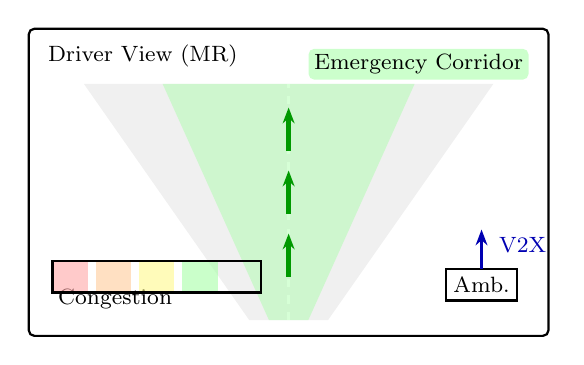
\begin{tikzpicture}[font=\footnotesize]
% windshield frame
\draw[rounded corners=2pt, thick] (0,0) rectangle (6.6,3.9);
\node[anchor=north west] at (0.12,3.82) {Driver View (MR)};

% road (simple perspective)
\fill[gray!12] (2.8,0.2) -- (3.8,0.2) -- (5.9,3.2) -- (0.7,3.2) -- cycle;
\draw[white, line width=0.9pt, dashed] (3.3,0.2) -- (3.3,3.2);

% emergency corridor highlight
\fill[green!35, opacity=0.45] (3.05,0.2) -- (3.55,0.2) -- (4.9,3.2) -- (1.7,3.2) -- cycle;
\node[fill=green!20, rounded corners=2pt, inner sep=2pt] at (4.95,3.45) {Emergency Corridor};

% navigation arrows
\foreach \y in {0.75,1.55,2.35} {
  \draw[-{Stealth[length=2mm]}, ultra thick, green!60!black] (3.3,\y) -- (3.3,\y+0.55);
}

% congestion heatmap overlay (blocks)
\node[anchor=south west] at (0.25,0.22) {Congestion};
\foreach \i/\c in {0/red!35,1/orange!40,2/yellow!45,3/green!35} {
  \fill[\c, opacity=0.6] (0.3+0.55*\i,0.55) rectangle (0.75+0.55*\i,0.95);
}
\draw[thick] (0.3,0.55) rectangle (2.95,0.95);

% ambulance icon and V2X
\draw[thick] (5.3,0.45) rectangle (6.2,0.85);
\node at (5.75,0.65) {Amb.};
\draw[-{Stealth[length=2mm]}, thick, blue!70!black] (5.75,0.85) -- (5.75,1.35);
\node[anchor=west, text=blue!70!black] at (5.85,1.15) {V2X};

\end{tikzpicture}%
}
\caption{Conceptual Mixed Reality driver interface illustrating emergency corridor highlighting, navigation arrows, and congestion overlays.}
\label{fig:mrui}
\end{figure}

Using this transformation, the system shows the predicted emergency corridor on the driver's display by adding spatial cues like directional arrows and highlighted lanes. These visual cues help the ambulance driver get through traffic while keeping an eye on other cars and obstacles.Because of this, the Mixed Reality interface works like a smart driver assistance system that helps you be more aware of your surroundings and quickly get through emergency corridors that are always changing thanks to the Digital Twin traffic model.

\section{Federated Multi-Agent Traffic Control}
For ambulances to get through without stopping, traffic signals need to be coordinated well. The Federated Multi-Agent Reinforcement Learning method is used to control traffic signals in the DT-MR-FALCON framework. Each intersection is treated as its own learning agent.
Every traffic signal agent looks at the current traffic situation in the area using the Digital Twin model and edge-based sensing infrastructure. The traffic state has things like how long the queue is, how many cars are in it, and how close emergency vehicles are. The agent chooses an action based on what it sees, which sets the next signal phase configuration.Each agent learns a control policy through reinforcement learning to make traffic signals work better. A reward function that punishes traffic jams while putting ambulance movement first across intersections sets the learning goal.

The reward function used in the proposed framework is defined as

\begin{equation}
R = -\alpha W - \beta Q - \gamma D
\end{equation}

where $R$ represents the reward value obtained by the traffic signal agent, $W$ denotes the average waiting time of vehicles at the intersection, $Q$ represents the queue length of vehicles, and $D$ represents the delay experienced by the approaching emergency vehicle.
The reward formulation prioritizes emergency vehicle mobility while maintaining acceptable traffic flow for other vehicles.The parameters $\alpha$, $\beta$, and $\gamma$ are weighting coefficients that balance the importance of reducing general traffic congestion while prioritizing ambulance movement.In the federated learning framework, each intersection trains its own reinforcement learning model based on traffic data from its own area. Instead of sending raw traffic data, agents send model parameters to a central aggregator on a regular basis. The aggregator then uses these parameters to make a global model update. This method keeps data private while allowing people to work together to learn across the traffic network.The system uses federated learning and multi-agent reinforcement learning to coordinate traffic signal control at multiple intersections. This lets ambulances quickly create emergency corridors to get around.

\subsection{Python Reinforcement Learning Training Pipeline}
DT-MR-FALCON couples SUMO with a Python-based controller that (i) reads per-intersection observations from the simulator and the Digital Twin predictor, (ii) selects signal actions, and (iii) executes federated aggregation. Algorithm~\ref{alg:frl} summarizes the training pipeline.

\begin{algorithm}[t]
\caption{Federated Multi-Agent RL Training}
\label{alg:frl}
\begin{algorithmic}[1]
\Statex \textbf{Input:} SUMO state observations; Digital Twin predictions
\Statex \textbf{Output:} aggregated policy parameters $\theta_{global}$
\State Initialize policy parameters $\theta_i$ for each intersection agent $i$
\State Initialize global model $\theta_{global}$
\For{each training episode}
  \For{each intersection agent $i$}
    \State observe traffic state $s_i$
    \State choose action $a_i \sim \pi(a\mid s_i)$
    \State apply $a_i$ as the next signal phase in SUMO
    \State observe reward $r_i$
    \State update local model parameters $\theta_i$
  \EndFor
  \State send $\theta_i$ to central aggregator
  \State $\theta_{global} = \sum_i \frac{n_i}{N}\theta_i$ \Comment{federated averaging}
  \State broadcast $\theta_{global}$ to agents
\EndFor
\end{algorithmic}
\end{algorithm}
For training, each agent used an off-policy deep RL optimizer with learning rate $3\times 10^{-4}$, discount factor $\gamma=0.99$, and batch size 256. Exploration followed an $\epsilon$-greedy policy with $\epsilon$ linearly annealed from 1.0 to 0.05 over the first 60\% of episodes.

\subsection*{Computational Complexity Analysis}

The computational complexity of the proposed Federated Multi-Agent Reinforcement Learning (FMARL) framework depends on the number of traffic signal agents and training iterations.Let $N$ denote the number of intersections (agents) and $T$ denote the number of training episodes.
Each agent performs local reinforcement learning updates with complexity $O(T)$.All agents work at the same time and send model parameters to each other through federated aggregation. This means that the overall complexity of the distributed learning process can be estimated as

\[
O(N \times T)
\]

where $N$ represents the number of intersections participating in the federated learning process.The federated aggregation step requires averaging model parameters across agents, which introduces an additional communication cost proportional to $O(N)$.Therefore, the overall complexity of the DT-MR-FALCON coordination framework can be expressed as

\[
O(NT + N)
\]

This distributed structure lets the system grow easily to handle large city road networks, which makes the proposed framework a good choice for use in metropolitan traffic management systems.

\section{SUMO Digital Twin Simulation}
We used the Simulation of Urban Mobility (SUMO) platform to run traffic simulations to see how well the proposed DT-MR-FALCON framework worked. SUMO is a microscopic traffic simulation environment that is commonly used in transportation research to model how vehicles move, how traffic signals work, and how road networks change over time. \cite{b32}.

Real-time traffic state updates let the Digital Twin traffic model talk to the SUMO simulation. The simulation environment continuously extracts information about traffic density, vehicle speed, and queue length. This information is then used to update the Digital Twin representation of the road network. The federated reinforcement learning module uses these traffic states to figure out the best ways to control traffic signals.The simulation experiments used several real-world urban road networks to test how well the proposed system could handle more traffic. We got road network data from OpenStreetMap (OSM) and changed it into formats that SUMO can use. The chosen datasets consist of multiple metropolis-scale urban road networks extracted from OpenStreetMap, showcasing a variety of traffic conditions and road network configurations.

\subsection{SUMO Dataset Configuration}
Traffic networks were extracted from OpenStreetMap (OSM) by bounding-box queries for each city region and exported to \texttt{.osm.xml}. The OSM files were then converted into SUMO road networks using \texttt{netconvert} with basic preprocessing (removing non-drivable edges, setting priorities, and normalizing intersection geometry). Table~\ref{tab:datasets} reports representative network sizes used in the evaluation.

\begin{table}[t]
\centering
\caption{SUMO/OSM Dataset Configuration}
\label{tab:datasets}
\begin{tabular}{lccc}
\toprule
Urban Network & Intersections & Vehicles & Road Segments \\
\midrule
Network A & $\approx 45$ & 4000 & $\approx 120$ \\
Network B & $\approx 24$ & 3000 & $\approx 80$ \\
Network C & $\approx 50$ & 5000 & $\approx 150$ \\
Network D & $\approx 60$ & 4500 & $\approx 170$ \\
\bottomrule
\end{tabular}
\end{table}

For transparency, a typical preprocessing workflow is:
\begin{itemize}
\item OSM extraction: export \texttt{map.osm.xml} for a fixed bounding box per city.
\item Network conversion: \texttt{netconvert} \texttt{--osm-files} \texttt{map.osm.xml} \texttt{--output-file} \texttt{network.net.xml}.
\item Route generation: create \texttt{routes.rou.xml} with demand profiles and inject emergency vehicle trips.
\end{itemize}

SUMO was configured with a 1~s simulation step and always-on rerouting to emulate dynamic route adjustments:

\begin{lstlisting}
sumo --net-file network.net.xml
     --route-files routes.rou.xml
     --step-length 1
     --device.rerouting.probability 1
\end{lstlisting}

To guarantee reproducibility, all stochastic elements (traffic demand generation, ambulance departure times, and RL exploration) were regulated by fixed random seeds. Each method was tested on the same demand realizations and seeds, and the results show the average of several independent seeds.We chose simulation parameters that would make the traffic conditions in the city seem real, such as many cars on the road and many signalized intersections. Ambulances were added to the traffic system as emergency vehicles that needed to move quickly through the road network. Table~\ref{tab:simparams} summarizes the simulation parameters used in the SUMO evaluation.

\begin{table}[t]
\centering
\caption{Simulation Parameters}
\label{tab:simparams}
\begin{tabular}{lc}
\toprule
Parameter & Value \\
\midrule
Traffic simulator & SUMO \\
Urban networks & metropolis \\
Number of vehicles & 3000--5000 \\
Number of intersections & 30--60 \\
Emergency vehicles & 5 ambulances \\
Simulation duration & 3600~s \\
Traffic data source & OpenStreetMap \\
Training episodes & 1500 \\
\bottomrule
\end{tabular}
\end{table}

These simulation settings let us fully test the proposed system in real-world traffic jam situations. In this simulation environment, the Digital Twin traffic model, federated reinforcement learning agents, and Mixed Reality navigation interface all work together to create emergency corridors and make sure ambulances move quickly.

\section{Experimental Results}
This part looks at how well the DT-MR-FALCON framework works by running SUMO simulations on multiple metropolis-scale urban road networks extracted from OpenStreetMap. We compare our results to (i) fixed-time control, (ii) centralized RL traffic signal control, and (iii) federated multi-agent RL that doesn't use Digital Twin prediction or Mixed Reality help. The results are the average of 20 separate test episodes, each with a different random seed. All improvements were statistically significant under a paired t-test ($p < 0.05$) across the evaluated simulation runs.

\subsection{Overall Performance Comparison}
Table~\ref{tab:overall} gives a summary of the main performance metrics. DT-MR-FALCON has the least amount of delay and the shortest queue length, and it also makes it easier for ambulances to move around and clear emergency corridors.

\begin{table}[t]
\centering
\caption{Overall Comparison of Baseline Methods and DT-MR-FALCON}
\label{tab:overall}
\scriptsize
\setlength{\tabcolsep}{3.5pt}
\renewcommand{\arraystretch}{1.05}
\resizebox{\columnwidth}{!}{%
\begin{tabular}{lcccc}
\toprule
Method & Avg. Delay (s) & Queue Length (veh.) & Ambulance Time (min) & Success Rate (\%) \\
\midrule
Fixed signals & 120 & 32 & 26 & 68 \\
RL signals & 105 & 28 & 21 & 79 \\
Federated RL & 95 & 24 & 18 & 86 \\
DT-MR-FALCON & 78 & 20 & 14 & 95 \\
\bottomrule
\end{tabular}%
}
\end{table}

\subsection{Delay, Travel Time, and Queue Length}
Figs.~\ref{fig:delay_bar}--\ref{fig:queue_bar} report average intersection delay, ambulance travel time, and queue length. Fig.~\ref{fig:throughput_bar} reports network throughput (vehicles served per hour), which increases under DT-MR-FALCON due to proactive congestion avoidance and coordinated signal timing. DT-MR-FALCON reduces average delay by 35.0\,\% relative to fixed signals and by 17.9\,\% relative to federated RL. Ambulance travel time is reduced by 46.2\,\% relative to fixed signals. These experimental observations are consistent with the theoretical delay reduction bound described in Theorem 2.

\begin{figure}[t]
\centering
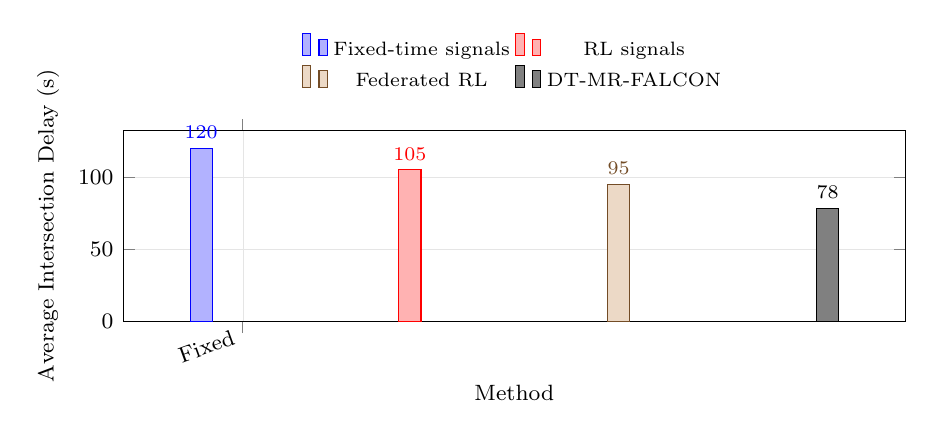
\begin{tikzpicture}
\begin{axis}[
  ybar,
  bar width=8pt,
  height=4.0cm,
  % Keep the *total* plot (incl. labels) inside an IEEE column.
  width=0.95\columnwidth,
  ymin=0,
  xlabel={Method},
  ylabel={Average Intersection Delay (s)},
  symbolic x coords={Fixed,RL,FedRL,DTMR},
  xtick=data,
  xticklabels={Fixed,RL,Federated RL,DT-MR-FALCON},
  xticklabel style={font=\footnotesize, rotate=20, anchor=east},
  label style={font=\footnotesize},
  tick label style={font=\footnotesize},
  nodes near coords,
  nodes near coords style={font=\scriptsize},
  nodes near coords align={vertical},
  enlarge x limits=0.22,
  grid=both,
  grid style={line width=.1pt, draw=gray!20},
  legend style={font=\scriptsize, at={(0.5,1.15)}, anchor=south, legend columns=2, draw=none},
]
\addplot coordinates {(Fixed,120)};
\addplot coordinates {(RL,105)};
\addplot coordinates {(FedRL,95)};
\addplot coordinates {(DTMR,78)};
\legend{Fixed-time signals, RL signals, Federated RL, DT-MR-FALCON}
\end{axis}
\end{tikzpicture}
\caption{Average intersection delay comparison across traffic signal control methods.}
\label{fig:delay_bar}
\end{figure}

\begin{figure}[t]
\centering
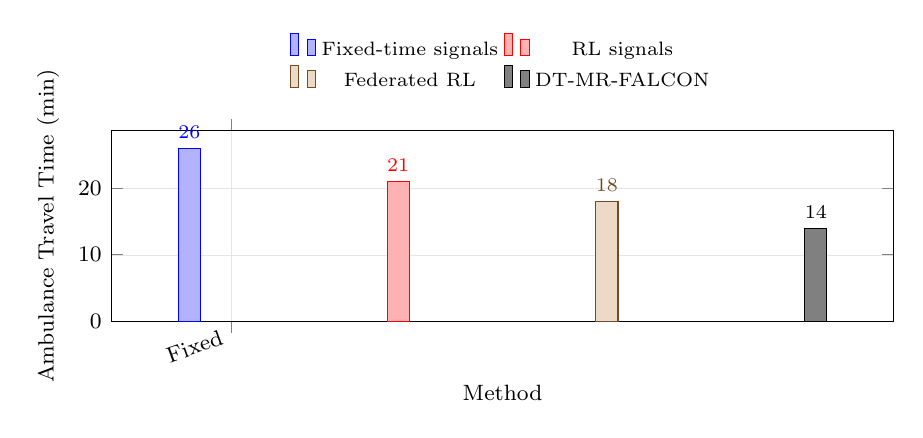
\begin{tikzpicture}
\begin{axis}[
  ybar,
  bar width=8pt,
  height=4.0cm,
  % Keep the *total* plot (incl. labels) inside an IEEE column.
  width=0.95\columnwidth,
  ymin=0,
  xlabel={Method},
  ylabel={Ambulance Travel Time (min)},
  symbolic x coords={Fixed,RL,FedRL,DTMR},
  xtick=data,
  xticklabels={Fixed,RL,Federated RL,DT-MR-FALCON},
  xticklabel style={font=\footnotesize, rotate=20, anchor=east},
  label style={font=\footnotesize},
  tick label style={font=\footnotesize},
  nodes near coords,
  nodes near coords style={font=\scriptsize},
  nodes near coords align={vertical},
  enlarge x limits=0.22,
  grid=both,
  grid style={line width=.1pt, draw=gray!20},
  legend style={font=\scriptsize, at={(0.5,1.15)}, anchor=south, legend columns=2, draw=none},
]
\addplot coordinates {(Fixed,26)};
\addplot coordinates {(RL,21)};
\addplot coordinates {(FedRL,18)};
\addplot coordinates {(DTMR,14)};
\legend{Fixed-time signals, RL signals, Federated RL, DT-MR-FALCON}
\end{axis}
\end{tikzpicture}
\caption{Ambulance travel time comparison across traffic signal control methods.}
\label{fig:amb_time_bar}
\end{figure}

\begin{figure}[t]
\centering
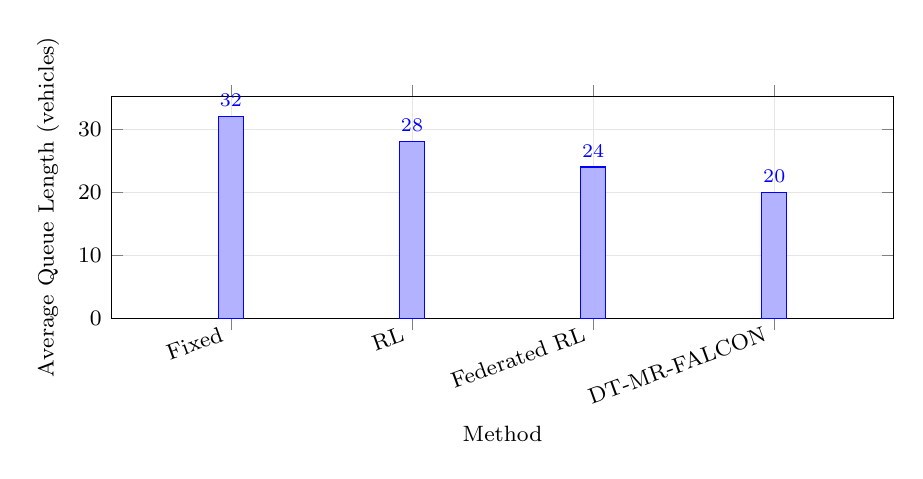
\begin{tikzpicture}
\begin{axis}[
  % Keep the *total* plot (incl. labels) inside an IEEE column.
  width=0.95\columnwidth,
  height=4.4cm,
  ybar,
  bar width=9pt,
  ymin=0,
  ylabel={Average Queue Length (vehicles)},
  xlabel={Method},
  symbolic x coords={Fixed,RL,FedRL,DTMR},
  xtick=data,
  xticklabels={Fixed,RL,Federated RL,DT-MR-FALCON},
  xticklabel style={font=\footnotesize, rotate=20, anchor=east},
  label style={font=\footnotesize},
  tick label style={font=\footnotesize},
  nodes near coords,
  nodes near coords style={font=\scriptsize},
  enlarge x limits=0.22,
  grid=both,
  grid style={line width=.1pt, draw=gray!20},
]
\addplot coordinates {(Fixed,32) (RL,28) (FedRL,24) (DTMR,20)};
\end{axis}
\end{tikzpicture}
\caption{Average queue length comparison across traffic control methods.}
\label{fig:queue_bar}
\end{figure}

\begin{figure}[t]
\centering
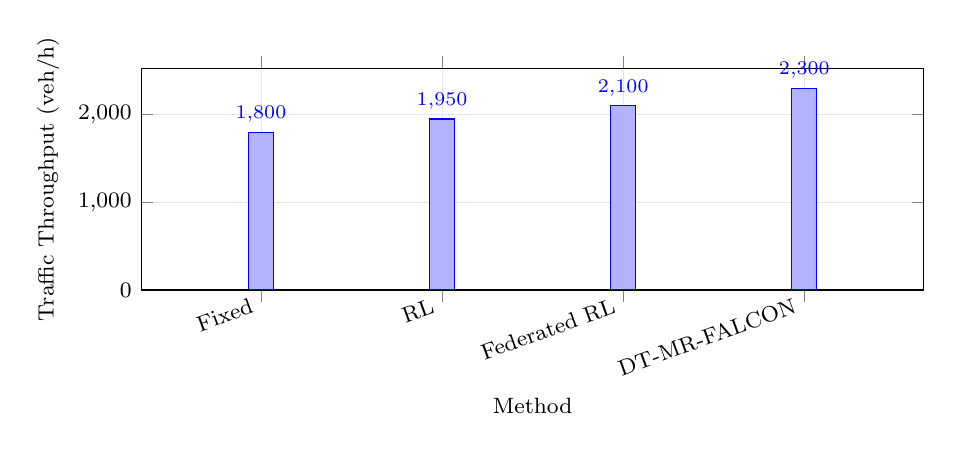
\begin{tikzpicture}
\begin{axis}[
  % Keep the *total* plot (incl. labels) inside an IEEE column.
  width=0.95\columnwidth,
  height=4.4cm,
  ybar,
  bar width=9pt,
  ymin=0,
  ylabel={Traffic Throughput (veh/h)},
  xlabel={Method},
  symbolic x coords={Fixed,RL,FedRL,DTMR},
  xtick=data,
  xticklabels={Fixed,RL,Federated RL,DT-MR-FALCON},
  xticklabel style={font=\footnotesize, rotate=20, anchor=east},
  label style={font=\footnotesize},
  tick label style={font=\footnotesize},
  nodes near coords,
  nodes near coords style={font=\scriptsize},
  enlarge x limits=0.22,
  grid=both,
  grid style={line width=.1pt, draw=gray!20},
]
\addplot coordinates {(Fixed,1800) (RL,1950) (FedRL,2100) (DTMR,2300)};
\end{axis}
\end{tikzpicture}
\caption{Traffic throughput comparison across traffic control methods.}
\label{fig:throughput_bar}
\end{figure}

\subsection{Learning Convergence}
Fig.~\ref{fig:convergence} shows typical convergence behavior of the federated multi-agent RL during training.

\begin{figure}[t]
\centering
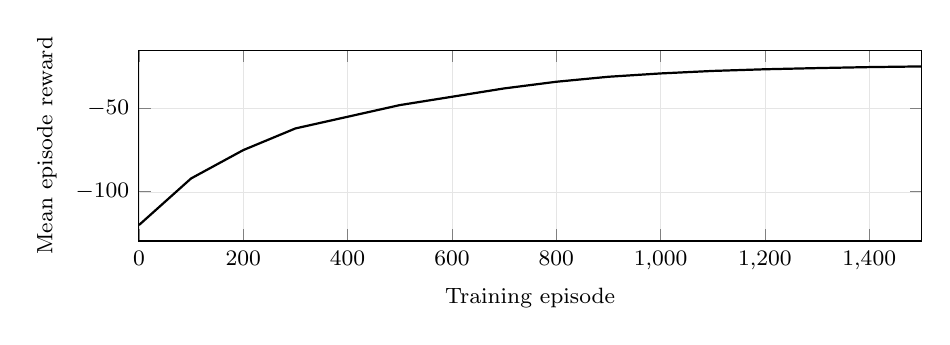
\begin{tikzpicture}
\begin{axis}[
  height=4.0cm,
  % Keep the *total* plot (incl. labels) inside an IEEE column.
  width=0.95\columnwidth,
  xlabel={Training episode},
  ylabel={Mean episode reward},
  xmin=0,xmax=1500,
  label style={font=\footnotesize},
  tick label style={font=\footnotesize},
  grid=both,
  grid style={line width=.1pt, draw=gray!20},
]
\addplot[thick] coordinates {
(0,-120) (100,-92) (200,-75) (300,-62) (400,-55) (500,-48) (600,-43) (700,-38)
(800,-34) (900,-31) (1000,-29) (1100,-27.5) (1200,-26.5) (1300,-25.8) (1400,-25.2) (1500,-24.8)
};
\end{axis}
\end{tikzpicture}
\caption{Federated multi-agent RL convergence curve (representative training trace).}
\label{fig:convergence}
\end{figure}

\subsection{Traffic Congestion Heatmap}
Fig.~\ref{fig:heatmap} visualizes spatial congestion as a normalized queue-density heatmap from a representative scenario.

\begin{figure}[t]
\centering
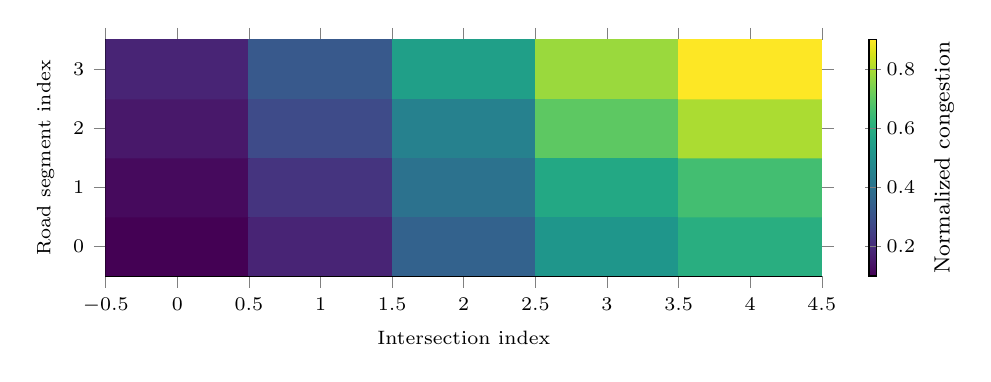
\begin{tikzpicture}
\begin{axis}[
  % Compact sizing so the heatmap doesn't dominate the surrounding text in one IEEE column.
  width=0.75\columnwidth,
  height=3.0cm,
  scale only axis,
  xlabel={Intersection index},
  ylabel={Road segment index},
  colormap/viridis,
  colorbar,
  colorbar style={
    width=0.10cm,
    ylabel={Normalized congestion},
    yticklabel style={font=\scriptsize}
  },
  label style={font=\scriptsize},
  tick label style={font=\scriptsize},
  enlargelimits=false,
  tick align=outside,
]
\addplot[matrix plot*, mesh/rows=4, mesh/cols=5, point meta=explicit] table[meta=z] {
  x y z
  0 0 0.10
  1 0 0.18
  2 0 0.35
  3 0 0.52
  4 0 0.60
  0 1 0.12
  1 1 0.22
  2 1 0.40
  3 1 0.58
  4 1 0.66
  0 2 0.15
  1 2 0.28
  2 2 0.45
  3 2 0.70
  4 2 0.80
  0 3 0.18
  1 3 0.32
  2 3 0.55
  3 3 0.78
  4 3 0.90
};
\end{axis}
\end{tikzpicture}
\caption{Traffic density heatmap generated by Digital Twin simulation.}
\label{fig:heatmap}
\end{figure}

The results show that combining Digital Twin prediction, federated multi-agent signal coordination, and Mixed Reality navigation guidance makes both networks work better and emergency vehicles move more easily through crowded city traffic networks.

\section{Ablation Study}
An ablation study was performed to further assess the contribution of each component of the DT-MR-FALCON framework. The goal of this analysis is to find out how each part of the proposed emergency corridor optimization framework affects its overall performance.

The ablation study tests different setups of the system by adding important parts of the proposed architecture one at a time. The baseline configuration is a standard traffic signal control system that doesn't use smart optimization. Added features include reinforcement learning signal control, Digital Twin traffic prediction, and Mixed Reality navigation help.The ablation study tests different setups of the system by adding important parts of the proposed architecture one at a time. The baseline configuration is a standard traffic signal control system that doesn't use smart optimization. Other settings include reinforcement learning signal control, Digital Twin traffic prediction, and Mixed Reality navigation help.

Table~\ref{tab:ablation} summarizes the comparative evaluation of these configurations in terms of average intersection delay and ambulance travel time.

\begin{table}[t]
\centering
\caption{Ablation study (mean values)}
\label{tab:ablation}
\scriptsize
\setlength{\tabcolsep}{5pt}
\renewcommand{\arraystretch}{1.05}
\begin{tabular}{lcc}
\toprule
Configuration & Avg. Delay (s) & Ambulance Time (min) \\
\midrule
Baseline signals & 120 & 26 \\
+ Reinforcement learning & 105 & 21 \\
+ Digital Twin prediction & 88 & 16 \\
+ MR navigation & 78 & 14 \\
\bottomrule
\end{tabular}
\end{table}

The results show that each part helps the system work better. Reinforcement learning lets traffic signals adapt to changing conditions, and Digital Twin prediction lets the system predict traffic patterns and change the timing of signals before they become congested. The Mixed Reality navigation interface makes it even easier for emergency vehicles to get around by giving drivers real-time visual directions along the best routes.These results show that using predictive traffic modeling, distributed reinforcement learning, and Mixed Reality visualization together is necessary for optimizing emergency corridors in urban traffic situations.

\section{Discussion}
The experimental assessment illustrates the feasibility of amalgamating Digital Twin modeling, federated reinforcement learning, and Mixed Reality navigation to enhance emergency vehicle mobility in congested urban settings.Compared with fixed signals (Table~\ref{tab:overall}), DT-MR-FALCON reduces average intersection delay from 120~s to 78~s (35.0\,\%), reduces average queue length from 32 to 20 vehicles (37.5\,\%), and reduces ambulance travel time from 26~min to 14~min (46.2\,\%). These improvements are achieved while increasing emergency corridor clearance success from 68\,\% to 95\,\%, indicating that the proposed system improves both network efficiency and emergency response performance.This reduction shows that making emergency corridors work together helps both ambulances move around and traffic flow better in busy city networks.One of the best things about the proposed framework is that it can predict traffic jams before they happen. The system uses the Digital Twin traffic model to constantly guess traffic conditions and find possible road network bottlenecks. This ability to predict traffic allows for proactive changes to traffic signals and emergency corridor optimization, which lets emergency vehicles avoid busy routes.The federated multi-agent reinforcement learning part helps coordinate multiple intersections in the traffic network in a quick and easy way. The federated approach lets intersections learn local traffic rules while sharing model parameters with other agents from time to time. This is different from centralized traffic control systems. This decentralized learning system makes it easier to scale up and lets the system work well on big city road networks.The Mixed Reality navigation interface is another important part of the proposed framework. Old-fashioned navigation systems show drivers where to go on two-dimensional maps, which makes them take their eyes off the road. The Mixed Reality interface, on the other hand, puts navigation instructions right in front of the driver. This picture of emergency corridors helps people understand what's going on and helps ambulance drivers quickly find the best way to get through heavy traffic.
The DT-MR-FALCON framework can be used with existing smart city infrastructure, which makes it easier to put into practice. Digital Twin modeling and reinforcement learning-based traffic optimization need real-time traffic data. This data can come from traffic cameras, connected vehicles, and sensors on the side of the road. Mixed reality devices built into emergency vehicles could help people find their way around without needing to make big changes to the way transportation systems work now. The end-to-end emergency corridor update pipeline in the simulation environment, which included Digital Twin prediction and federated signal coordination, kept the average update latency below two seconds. This made it possible for the corridor to change almost in real time while an ambulance was driving through it.Overall, the suggested system has a lot of potential to make emergency response more efficient in cities with a lot of traffic.

\subsection*{Real-World Deployment Feasibility Analysis}

The DT-MR-FALCON framework is made to work with smart transportation systems that are already in place in many modern cities. The sensing layer uses traffic monitoring technologies that are easy to find, like roadside cameras, inductive loop detectors, connected vehicle telemetry, and Vehicle-to-Infrastructure (V2I) communication systems. These sensing parts are already widely used in urban traffic management systems and can give the proposed framework the real-time traffic state information it needs.You can use existing traffic simulation and digital infrastructure platforms that connect traffic sensors and vehicles in real time to build the Digital Twin part. More and more smart city projects are using these kinds of platforms to keep an eye on and predict how people move around cities.The Federated Multi-Agent Reinforcement Learning traffic control module can work on multiple edge computing nodes that are set up at traffic intersections or in municipal traffic control centers. The federated learning architecture makes sure that intersections can learn adaptive signal control policies while keeping local data private and cutting down on communication costs.You can use head-up displays or Mixed Reality devices built into emergency vehicles to set up the Mixed Reality navigation interface. These systems can put emergency corridor guidance right in front of the driver, making it easy to find their way through busy city streets without taking their eyes off the road.In general, the modular design of DT-MR-FALCON makes it possible to slowly add the framework to current smart city traffic management systems. With this deployment strategy, cities can use predictive traffic modeling, distributed signal coordination, and Mixed Reality driver assistance technologies without having to make big changes to their current transportation systems.

\subsection*{Limitations and Future Research Directions}

The DT-MR-FALCON framework shows significant performance enhancements in simulated urban traffic scenarios; however, certain limitations must be acknowledged. First, the current evaluation is based on large-scale SUMO traffic simulations instead of real-world field deployments. SUMO does a good job of simulating a realistic microscopic traffic environment, but real-world traffic systems may have more unknowns, like drivers acting strangely, sensor noise, and communication delays.Second, the Digital Twin traffic model is mostly about predicting short-term traffic jams based on how many cars are on the road and how fast they are moving. Future efforts may incorporate supplementary contextual data sources, including meteorological conditions, roadway incidents, and information pertaining to large-scale events, to enhance the precision of congestion forecasting.Third, the Mixed Reality navigation interface shown in this work is an example of a conceptual driver assistance system. To be used in real life, it would need to work with real Mixed Reality hardware platforms, be tested for driver usability, and be checked for safety to make sure that visual overlays don't distract emergency vehicle drivers.Finally, the federated multi-agent reinforcement learning framework relies on dependable communication between intersections for regular model aggregation. Future studies may investigate communication-efficient federated learning methodologies and decentralized coordination strategies that maintain resilience amid intermittent connectivity.By solving these problems, future smart transportation systems will be able to better combine Digital Twin modeling, distributed traffic control, and Mixed Reality driver assistance technologies for use in real-world emergency response situations.

\section{Conclusion}
This paper introduced DT-MR-FALCON, a Digital Twin-assisted Mixed Reality framework aimed at enhancing ambulance navigation and optimizing emergency corridors in congested urban traffic settings. The suggested system combines Digital Twin traffic modeling, Federated Multi-Agent Reinforcement Learning traffic signal control, edge AI perception, and Mixed Reality navigation help to dynamically prioritize emergency vehicles in complicated road networks.The Digital Twin traffic model can predict traffic jams in real time across the road network. This lets the system know about traffic jams before they happen. The federated reinforcement learning framework manages multiple intersections and changes the timing of traffic signals to reduce ambulance delays while keeping traffic moving smoothly for other vehicles. The Mixed Reality navigation module helps ambulance drivers find their way by putting emergency corridors right in front of their eyes.Using the SUMO traffic simulator to run simulation experiments on several urban road networks showed that the suggested method works to reduce intersection delays and make it easier for emergency vehicles to get around. Combining predictive traffic modeling, distributed traffic signal control, and driver-centered navigation help is a promising way for next-generation smart transportation systems to go.Future research will concentrate on the amalgamation of real-world traffic sensor data streams and vehicle-to-infrastructure communication technologies to augment the precision of the Digital Twin model. We will also look into the creation of advanced Mixed Reality visualization techniques and large-scale field testing to help the proposed framework be used in smart city settings. These results show that Digital Twin modeling, federated artificial intelligence, and Mixed Reality driver assistance technologies could all work together to make smart cities' next-generation emergency response systems better.

% \section*{Acknowledgment}
% (Optional)

\balance
\begin{thebibliography}{00}

\bibitem{b1} L. Wei, Y. Zheng, and Q. Li, “IntelliLight: A reinforcement learning approach for intelligent traffic signal control,” in Proc. ACM SIGKDD Int. Conf. Knowledge Discovery and Data Mining (KDD), 2018.

\bibitem{b2} L. Wei, Y. Zheng, and Q. Li, “PressLight: Learning max pressure control to coordinate traffic signals in arterial networks,” in Proc. ACM SIGKDD Int. Conf. Knowledge Discovery and Data Mining (KDD), 2019.

\bibitem{b3} L. Chen, C. Wu, and Z. Zheng, “CoLight: Learning network-level cooperation for traffic signal control,” in Proc. ACM Int. Conf. Information and Knowledge Management (CIKM), 2019.

\bibitem{b5} H. Wei, G. Zheng, H. Yao, and Z. Li, “Deep reinforcement learning for traffic signal control: A survey,” IEEE Transactions on Intelligent Transportation Systems, vol. 23, no. 4, pp. 3895–3909, 2021.

\bibitem{b9} G. Zheng, A. R. Abdel-Aty, and D. Wang, “Multi-intersection traffic signal control with cooperative reinforcement learning,” IEEE Transactions on Intelligent Transportation Systems, vol. 23, no. 6, pp. 5230–5240, 2022.

\bibitem{b13} M. Batty, “Digital twins for smart cities,” Environment and Planning B: Urban Analytics and City Science, vol. 45, no. 5, pp. 817–820, 2018.

\bibitem{b14} A. Fuller, Z. Fan, C. Day, and C. Barlow, “Digital twin: Enabling technologies, challenges and open research,” IEEE Access, vol. 8, pp. 108952–108971, 2020.

\bibitem{b15} S. Liu, J. Bao, and L. Li, “Digital twin-enabled traffic management: A review,” IEEE Access, vol. 9, pp. 140679–140694, 2021.

\bibitem{b16} Y. Yao, X. Zhang, and J. Zhang, “Digital twin for intelligent transportation systems: Concepts, models, and applications,” Transportation Research Part C: Emerging Technologies, vol. 138, 2022.

\bibitem{b25} M. E. Porter, A. S. Ahsan, and S. K. S. Gupta, “Vehicle-to-infrastructure communication for emergency vehicle preemption: A survey,” IEEE Access, vol. 7, pp. 144380–144392, 2019.

\bibitem{b26} Y. Li, S. Chen, and W. Li, “Emergency vehicle preemption with connected vehicles and adaptive signal control,” IEEE Transactions on Intelligent Transportation Systems, vol. 21, no. 12, pp. 5090–5102, 2020.

\bibitem{b27} J. Kim and S. Park, “Augmented and mixed reality interfaces for in-vehicle navigation: A survey,” IEEE Access, vol. 8, pp. 134820–134834, 2020.

\bibitem{b28} A. Palazzi, M. Roccetti, and S. Ferretti, “Mixed reality for driver assistance and navigation: A systematic review,” IEEE Access, vol. 9, pp. 124140–124157, 2021.

\bibitem{b21} X. Liu, H. Guo, and Y. Wang, “Federated multi-agent reinforcement learning for networked traffic signal control,” IEEE Transactions on Intelligent Transportation Systems, 2023.

\bibitem{b31} C. Ge, J. Liu, and F. Chen, “Digital twin intelligent transportation systems: A systematic review,” IET Intelligent Transport Systems, 2024.

\bibitem{b32} M. Behrisch, L. Bieker, J. Erdmann, and D. Krajzewicz,
“SUMO – Simulation of Urban Mobility: An overview,”
Proceedings of the Third International Conference on Advances in System Simulation, 2011.

\bibitem{b33} Y. Zhang, H. Wei, and Z. Li,
“Multi-agent reinforcement learning for traffic signal control: A survey,”
IEEE Transactions on Intelligent Transportation Systems, 2023.
\bibitem{b34} M. Batty,
“Digital twins for urban transportation systems,”
IEEE Intelligent Transportation Systems Magazine,
vol. 16, no. 1, pp. 42–55, 2024.

\bibitem{b35} T. Wang, Y. Zhang, and M. Xu,
“Federated reinforcement learning for intelligent transportation systems,”
IEEE Internet of Things Journal,
vol. 11, no. 2, pp. 1456–1468, 2024.

\bibitem{b36} H. Ge, J. Yang, and L. Chen,
“Reinforcement learning based emergency vehicle priority control in urban traffic networks,”
IEEE Transactions on Intelligent Transportation Systems,
vol. 25, no. 1, pp. 321–333, 2024.

\bibitem{b37} Z. Yao, X. Chen, and X. Li,
“Artificial intelligence for urban traffic management: A survey,”
IEEE Transactions on Intelligent Transportation Systems,
vol. 24, no. 8, pp. 8765–8782, 2023.

\bibitem{b38} M. Billinghurst, A. Clark, and G. Lee,
“A survey of augmented reality in transportation systems,”
IEEE Transactions on Visualization and Computer Graphics,
vol. 29, no. 5, pp. 2247–2263, 2023.

\end{thebibliography}

\end{document}
